A software tool named the ``Kitting Viewer'' has been developed that
simulates the execution of a plan (CRCL command file) for changing a
kitting workstation from an initial state to a goal state. Usually, that is
a plan for making one or more kits. The Kitting Viewer evaluates the plan
as it runs. The Kitting Viewer source code is in C++ with OpenGL graphics.

\subsection{Overview}

The Kitting Viewer reads files describing the initial state, the goal state,
and the plan for getting from the initial state to the goal state.
Optionally, it also reads a scoring file. If no scoring file is specified
by the user, a hard-coded default scoring file structure is used. The
Kitting Viewer simulates execution of the plan, displays a view of the plan
being executed, and produces and displays metrics about the plan. All of
the metrics are numbers. All but one of the metrics are objective and
require no human judgement. These metrics are presented in
Section \ref{sect:Metrics}. The final metric is a subjective combination of
the other metrics in which the other metrics are weighted and combined as
specified by the scoring file. The scoring file may be edited as desired by
the user. Scoring details are given in Section \ref{sect:Scoring}.

The Kitting Viewer runs in two phases. In the first phase, each time the
user gives a signal (presses the \tt g \rm key) the next command from the
command file is executed. The Kitting Viewer may decide that a command
cannot be executed, but if it decides a command can be executed, it assumes
the command is executed properly. In the second phase, which starts after
all commands have been executed, each time the user gives a signal the
position of the next movable object in the goal file is checked.

Figure~\ref{fig:KittingViewer} shows the Kitting Viewer windows as they look
after a test run has been completed. The display uses three windows,
labeled Metrics \& Settings, Kitting Viewer, and Kitting Command \&
Messages. The windows may be moved and re-sized independently, like other
windows in a typical windowing system.

In Figure~\ref{fig:KittingViewer}, the large blue object is a work table.
The small blue object is the end effector changing station. The three empty
small green boxes are parts trays that formerly held parts. The large green
box on the left is a container for completed kits; it contains one kit. The
large empty green box on the right formerly held an empty kit tray.

The Kitting Viewer window shows a 3D animated color view of the kitting
workstation. The floor of the workstation is covered with a grid. The robot
in the workstation is represented by a gantry robot spanning the entire
width of the workstation. The gantry robot moves when any CRCL motion
command is executed. The speed at which the picture of the robot is
animated matches the actual commanded speed of the robot. Objects in the
workstation move if the robot moves them. The view in the window may be
translated, rotated, or zoomed at any time.

In the first phase of running the Kitting Viewer, the Kitting Command \&
Messages window shows the currently executing command or the most recently
executed command, if no command is currently executing. In the second
phase, the window shows messages describing success or failure in locating
goal objects.

The Metrics \& Settings window shows 12 (first phase) or 15 (second phase)
metrics at the top. Below that it shows 13 robot settings and two
Kitting Viewer settings. All but two of the robot settings correspond to
items that may be set using CRCL commands. The extra two are the
robot\rq{}s maximum speed and maximum acceleration, which may not be
reset. As commands are executed, metrics and settings are updated in the
window.
\begin{figure}[ht!]
\begin{center}
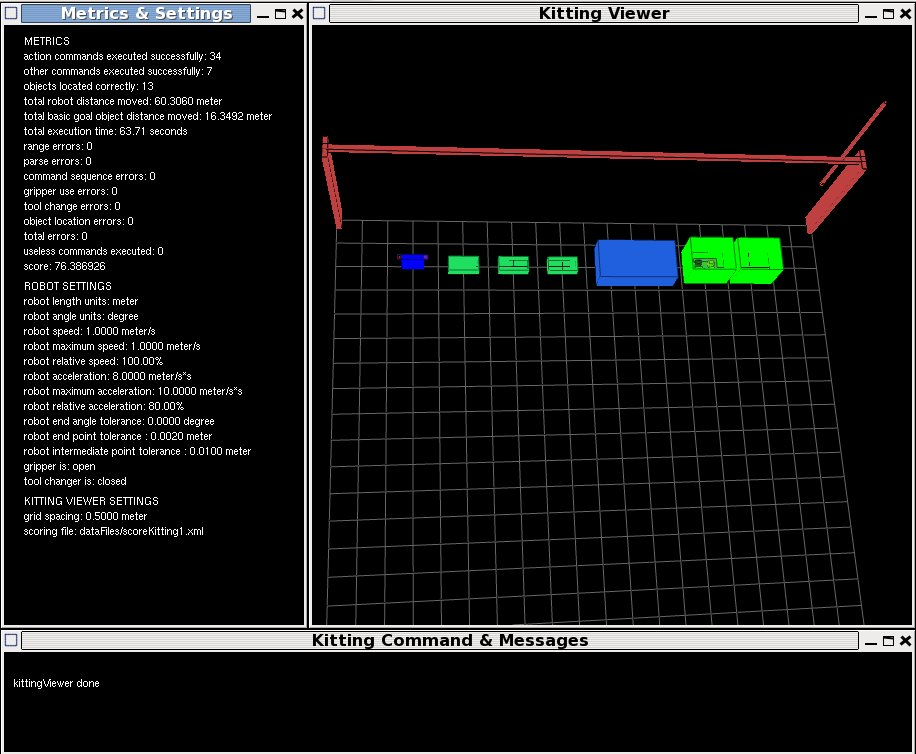
\includegraphics[width=8.5cm]{images/kittingViewer2013Feb23.jpg}
\caption{Kitting Viewer Display}
\label{fig:KittingViewer}
\end{center}
\end{figure}

\subsection{Errors}
In order to fully evaluate a plan file, usually, if a plan error is
detected, an error is recorded, but the Kitting Viewer continues to operate.
A few errors are fatal.
  
When the command parser encounters a line that it cannot parse, it adds
an \sf UnreadableMsg \rm to the list of commands it has parsed. The \sf
UnreadableMsg \rm includes the text of the line on which the parse error
occurred. When the \sf UnreadableMsg \rm is executed, the value of parse
errors is increased by one and the \sf UnreadableMsg \rm is displayed in
the Kitting Command \& Messages window so the user can see the line that
caused the problem.
  
\subsection{Controlling The Kitting Viewer}
Controlling the Kitting Viewer is accomplished by using the mouse and single
keys on the keyboard. When the Kitting Viewer starts up, a set of one-line
instructions is printed in the terminal window from which the
Kitting Viewer was started. Those instructions have the same meaning as
the longer explanations given below.

\begin{itemize}

\item \tt r \rm key -- the \tt r \rm key toggles the behavior of the
left mouse button between translating and rotating the picture. This is
needed so two-button mice will work.

\item Left mouse button -- By default, the left mouse button is used to
translate the picture.

\item Middle mouse button -- The middle mouse button is used to rotate the
picture.

\item Right mouse button -- The right mouse button is used to zoom in or
  out.

\item \tt h \rm key -- If the \tt h \rm key is pressed, the view in the
Kitting Viewer window returns to its original position.

\item \tt g \rm key -- If the \tt g \rm key is pressed when the plan is not
completely executed and no command is executing, the next command in the
plan is executed. If the \tt g \rm key is pressed when a command is in
progress, it has no effect. If the \tt g \rm key is pressed when the plan
is completely executed but not all goal objects have been checked, the
position of the next goal object is checked.

\item \tt t \rm key -- If the \tt t \rm key is pressed, a combined image of
all the windows will be saved in a file. The name of the file will be
kittingViewer\_N.ppm, where N starts at 0000 and increases by 1 each time
the t key is pressed. The ppm (portable pixmap) format is a common graphics
format that many graphics utilities can handle.

\item \tt z \rm or \tt q \rm key -- if the \tt z \rm or \tt q \rm key is
pressed, the Kitting Viewer program exits, and the windows disappear.

\end{itemize}

\subsection{Modeling}
The project in which the Kitting Viewer was developed has modeled the state
of a kitting workstation in both OWL and XML schema language. The XML model
is kitting.xsd. An automatic code generator named the GenXMiller written by
the authors at NIST is being used in the project. The GenXMiller will read
an XML schema and produce C++ classes and a parser for XML data files
corresponding to the XML schema. The GenXMiller was used to produce the C++
class model of a kitting workstation and the state file parser used in the
Kitting Viewer. The initial and goal state files used by the Kitting Viewer
are XML data files corresponding to the kitting.xsd XML schema.

The Kitting Viewer does a great deal of modeling while it runs. When the
initial state file is read, a model of the initial state is built and saved
as the current state of the workstation. A model of the goal state is also
built and saved. As the Kitting Viewer runs and CRCL commands are executed,
the Kitting Viewer determines the effect of executing each command on the
current state and updates it. The second phase of Kitting Viewer operation
compares the evolved current state with the goal state.

The logic of state changes is complex in some cases. The most interesting
cases involve what to do when executing CloseGripper and OpenGripper
commands. Details for CloseGripper are given below. 

A key issue is that composite objects may go out of existence or come into
existence while kits are being built. A kitting workstation builds kits.
The kits do not exist in the initial state but they do exist in the goal
state, so it is necessary to make them start to exist at some point in the
process. The initial state includes parts trays with parts. When all the
parts are removed from a parts tray with parts, it goes out of existence.
Of course the parts tray remains, but it is no longer a component of a
parts tray with parts. In the Kitting Viewer, a kit comes into existence
when the first part is placed in a kit tray, and a parts tray with parts
goes out of existence when the last part is removed from it.

For CloseGripper, if all of the following hold:
\newcounter{ifcount}
\begin{list}{\arabic{ifcount}.}%
{\usecounter{ifcount}}

\item  The robot is holding an end effector.

\item  The end effector is a single cup vacuum gripper (that's the only
   kind of gripper the Kitting Viewer knows how to use).

\item Either:\\
3A. There is a parts tray or kit tray with a topless boxy shape
    such that the gripper cup is within 0.1 mm of the bottom of the
    tray and is within 1 mm of the XY location of the origin of the tray. OR\\
3B. There is a part with a boxy shape with top such that the gripper cup
    is within 0.1 mm of the top of the part and is within 1 mm of the XY
    location of the middle of the top of the part.

\item The gripper is able to pick up that type of part or tray.

\item The Z axis of the gripper is 0,0,-1 and the Z axis of the object is
    0,0,1.

\item The gripper is open (implying the gripper is not holding anything).

\end{list}

Then the gripper will attach to an object. Call it B.

\begin{itemize}

\item If 3B above occurred, then B is a part

\item If 3A above occurred with a parts tray in a parts tray with parts,
   then B is the parts tray with parts.

\item If 3A above occurred with a parts tray not in a parts tray with parts,
   then B is the parts tray.

\item If 3A above occurred with a kit tray in a kit, then B is the kit.

\item If 3A above occurred with a kit tray not in a kit, then B is the kit tray.

\end{itemize}

When the gripper attaches to an object, the primary state changes (i.e.
changes in states present in kitting.xsd) are that the gripper is closed,
and the pose of the object is changed so that the object is located
relative to the gripper. In addition, as described above, if the object is
the last part in a parts tray with parts, the parts tray with parts will go
out of existence. The Kitting Viewer has several other state variables for
positions to make its work more efficient, and these are also updated.

